% =============================================================================
% Experiments section — structured for clarity (utility / q / bins).
%
% Sized for NeurIPS \textbf{one-column} (e.g.\ \texttt{neurips\_2024} with the
% \texttt{onecolumn} option): figures use full \verb|\linewidth| with strict
% \verb|\textheight| caps so stacked panels stay within roughly one text block.
%
% Preamble (suggested): \usepackage{graphicx,booktabs}
% Optional: \usepackage{caption} then \captionsetup{font=small,labelfont=bf}
% Run plot script to refresh assets:
%   python scripts/plot_headline_results.py --data-dir <headline_jsonl> \\
%       --out-dir paper/figures/experiments --fixed-k 8
%
% Paths assume \jobname.tex lives in paper/ (same folder as figures/).
%
% Float control (optional): \usepackage{placeins} then \FloatBarrier after
% each subsection if figures still pile at the top. For strict in-text
% placement of selected floats: \usepackage{float} and \begin{figure}[H].
% =============================================================================

\section{Experiments}
\label{sec:experiments}

We study transductive node classification with the same two-layer subgraph GCN everywhere.
Hyperparameters include: number of bins $K \in \{4,8,16\}$, single-phase training-node sampling rate $q \in \{0.05,0.10\}$, gradient clip $C{=}1$, Gaussian noise multiplier $\sigma/C$, and PRV accounting at $\delta{=}10^{-5}$ (reported~$\varepsilon$).
Full-graph GCN/MLP baselines are omitted from this draft; where helpful we compare against the \emph{non-DP subgraph} runs (Algo.~2 and~3 without noise) so partitioning and subsampling effects are isolated from privacy noise.

% ---------------------------------------------------------------------------
\subsection{Utility without differential privacy}
\label{sec:exp-nondp}

We first measure \emph{partitioning cost} when no DP mechanism is applied: same optimizer and early-stopping protocol, but no per-step clipping or noise.
Figure~\ref{fig:utility-nondp} shows test accuracy versus~$K$ for Algo.~2 (internal edges per bin) and Algo.~3 (same with dummy-bin dropout $p{=}0.3$).

\begin{figure}[htbp]
  \centering
  % One column: full width, low height cap (NeurIPS pages are short).
  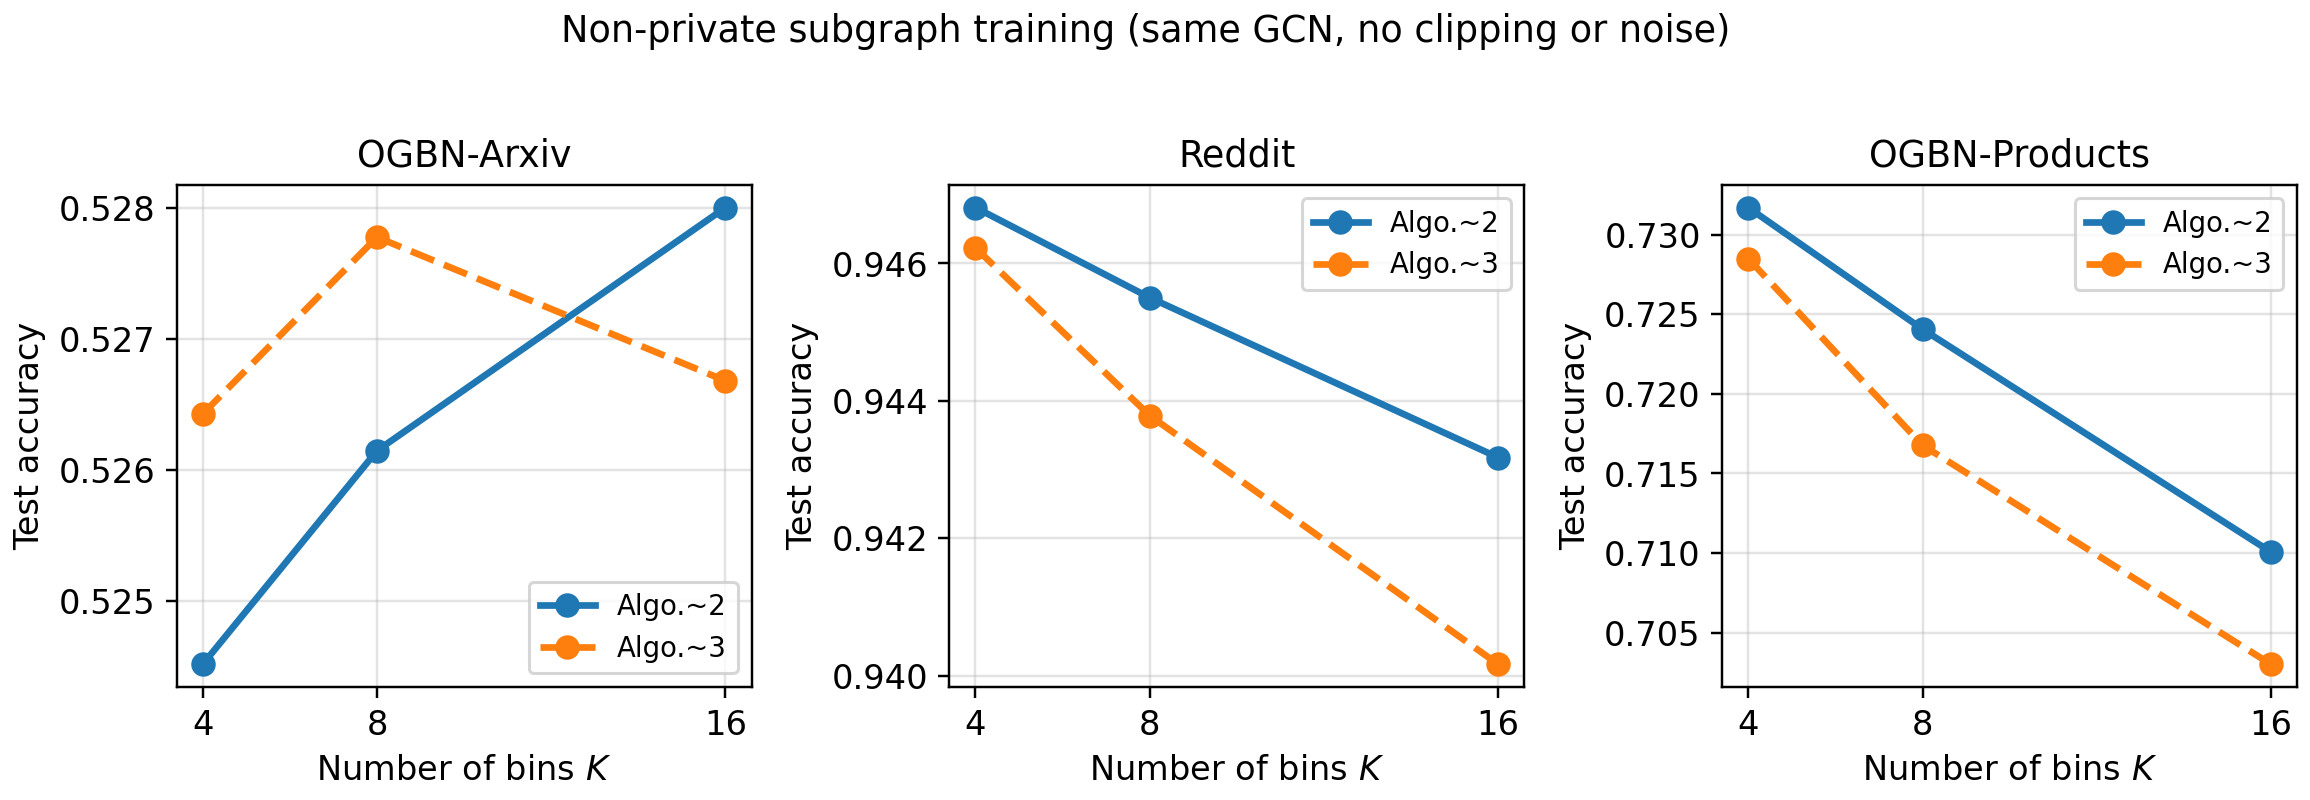
\includegraphics[width=\linewidth,height=0.22\textheight,keepaspectratio]{figures/experiments/utility_nondp.png}
  \caption{Non-private subgraph training: test accuracy vs.\ $K$ on the three benchmarks. Solid $=$ Algo.~2; dashed $=$ Algo.~3.}
  \label{fig:utility-nondp}
\end{figure}

Table~\ref{tab:nondp-utility} lists the same numbers (means over seeds when multiple logs exist).

\begin{table}[htbp]
  \centering
  \footnotesize
  \setlength{\tabcolsep}{5pt}
  \caption{Non-DP subgraph test accuracy (mean over seeds). Only $K\in\{4,8,16\}$.}
  \label{tab:nondp-utility}
  \begin{tabular}{lccc}
\toprule
Dataset & $K$ & Algo.~2 & Algo.~3 \\
\midrule
\texttt{ogbn-arxiv} & 4 & 0.525 & 0.526 \\
\texttt{ogbn-arxiv} & 8 & 0.526 & 0.528 \\
\texttt{ogbn-arxiv} & 16 & 0.528 & 0.527 \\
\texttt{reddit} & 4 & 0.947 & 0.946 \\
\texttt{reddit} & 8 & 0.946 & 0.944 \\
\texttt{reddit} & 16 & 0.943 & 0.940 \\
\texttt{ogbn-products} & 4 & 0.732 & 0.728 \\
\texttt{ogbn-products} & 8 & 0.724 & 0.717 \\
\texttt{ogbn-products} & 16 & 0.710 & 0.703 \\
\bottomrule
\end{tabular}

\end{table}

% ---------------------------------------------------------------------------
\subsection{Differential privacy and sampling rate~$q$}
\label{sec:exp-dp-q}

Under DP we use single-phase Poisson subsampling of training nodes with per-step inclusion probability~$q$.
To avoid overcrowded curves, the \emph{main} DP figures fix $K{=}8$ and show only four trajectories: Algo.~2 vs.\ Algo.~3, each at $q\in\{0.05,0.10\}$, with noise multiplier on the horizontal axis (top panel) and PRV~$\varepsilon$ on the horizontal axis (bottom panel).
A dotted line marks the best non-DP subgraph accuracy from Section~\ref{sec:exp-nondp}.

Table~\ref{tab:dp-q} summarizes a \emph{scalar} comparison at $\sigma/C{=}1$ and $K{=}8$: how much tightening~$q$ from $0.10$ to $0.05$ buys in~$\varepsilon$ at similar accuracy.

\begin{figure}[htbp]
  \centering
  % Stacked panels: full column width; height cap is the binding constraint.
  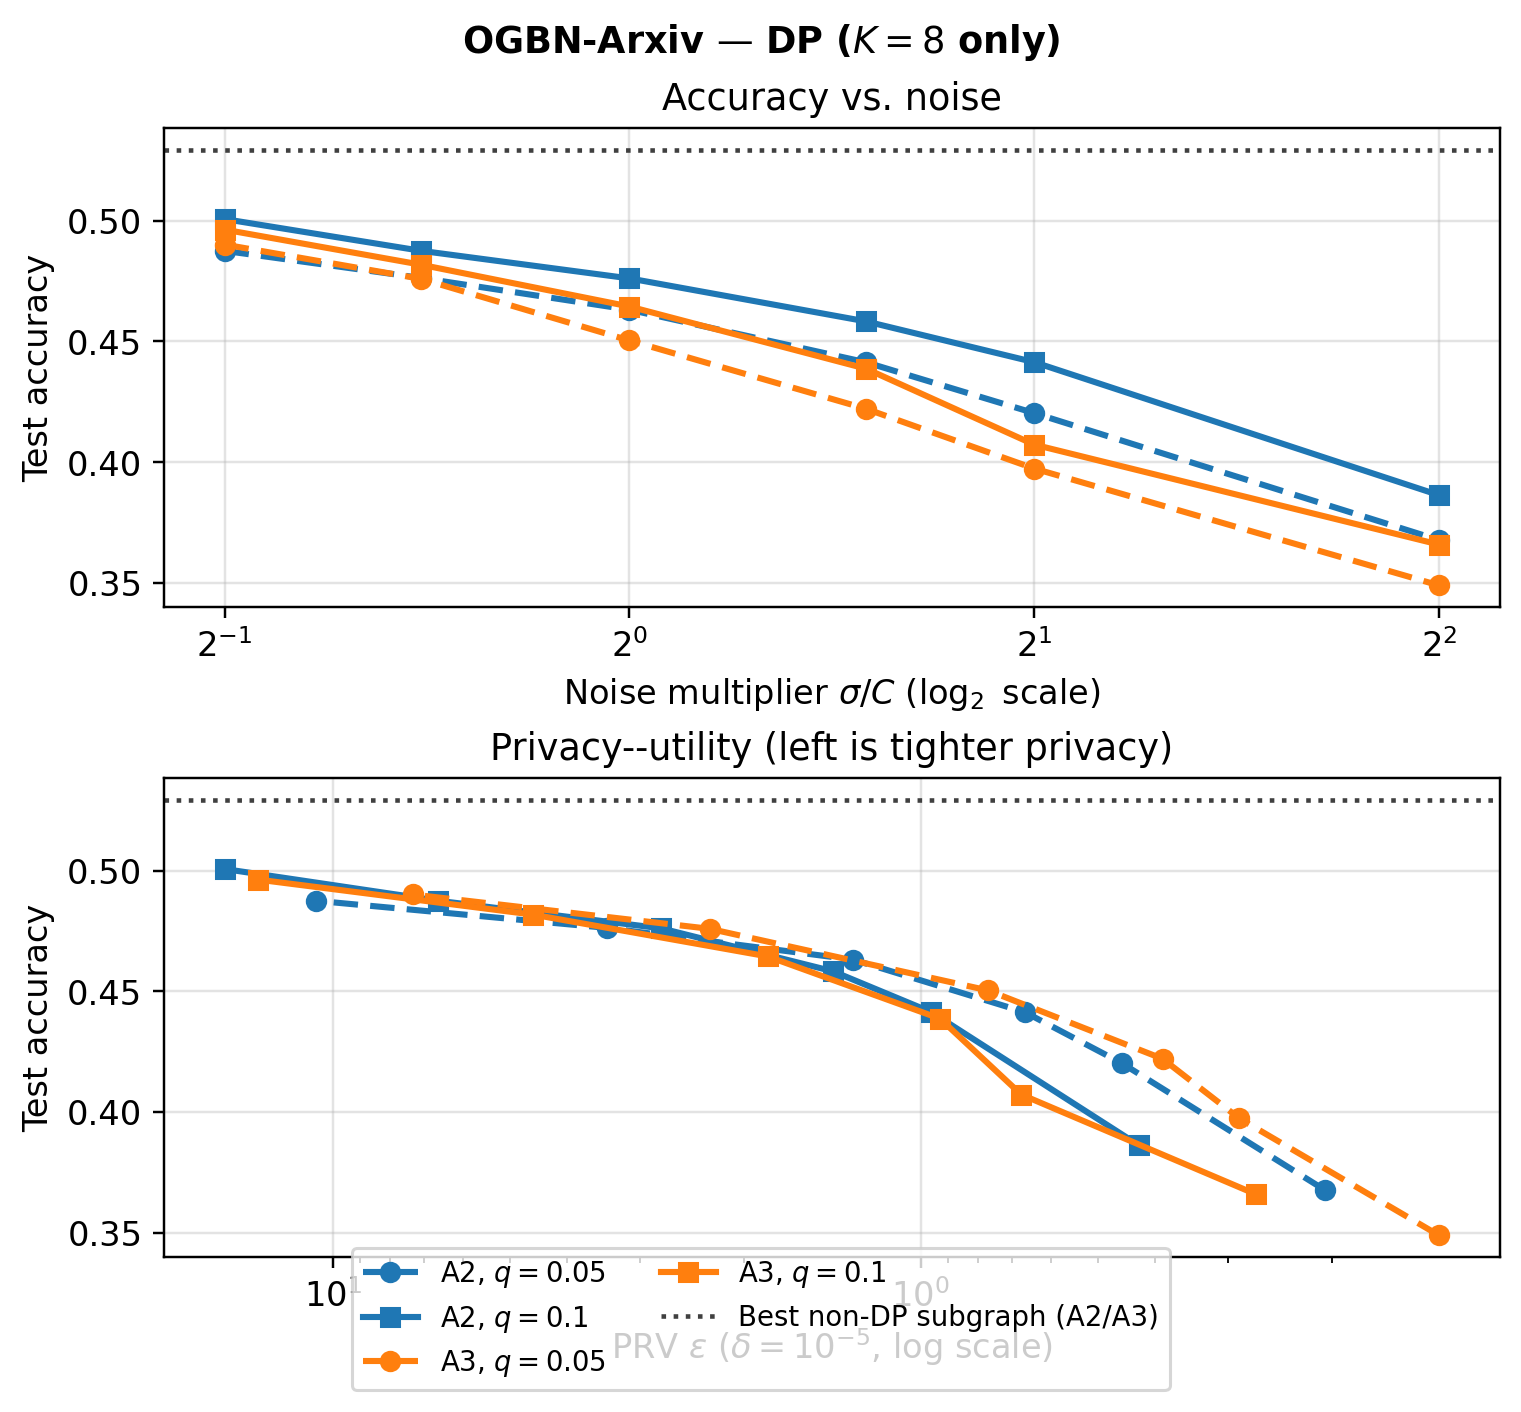
\includegraphics[width=\linewidth,height=0.30\textheight,keepaspectratio]{figures/experiments/dp_K8_ogbn_arxiv.png}
  \caption{\textbf{OGBN-Arxiv, $K{=}8$.} DP test accuracy vs.\ noise (top) and vs.\ PRV $\varepsilon$ (bottom).}
  \label{fig:dp-k8-arxiv}
\end{figure}

\begin{figure}[htbp]
  \centering
  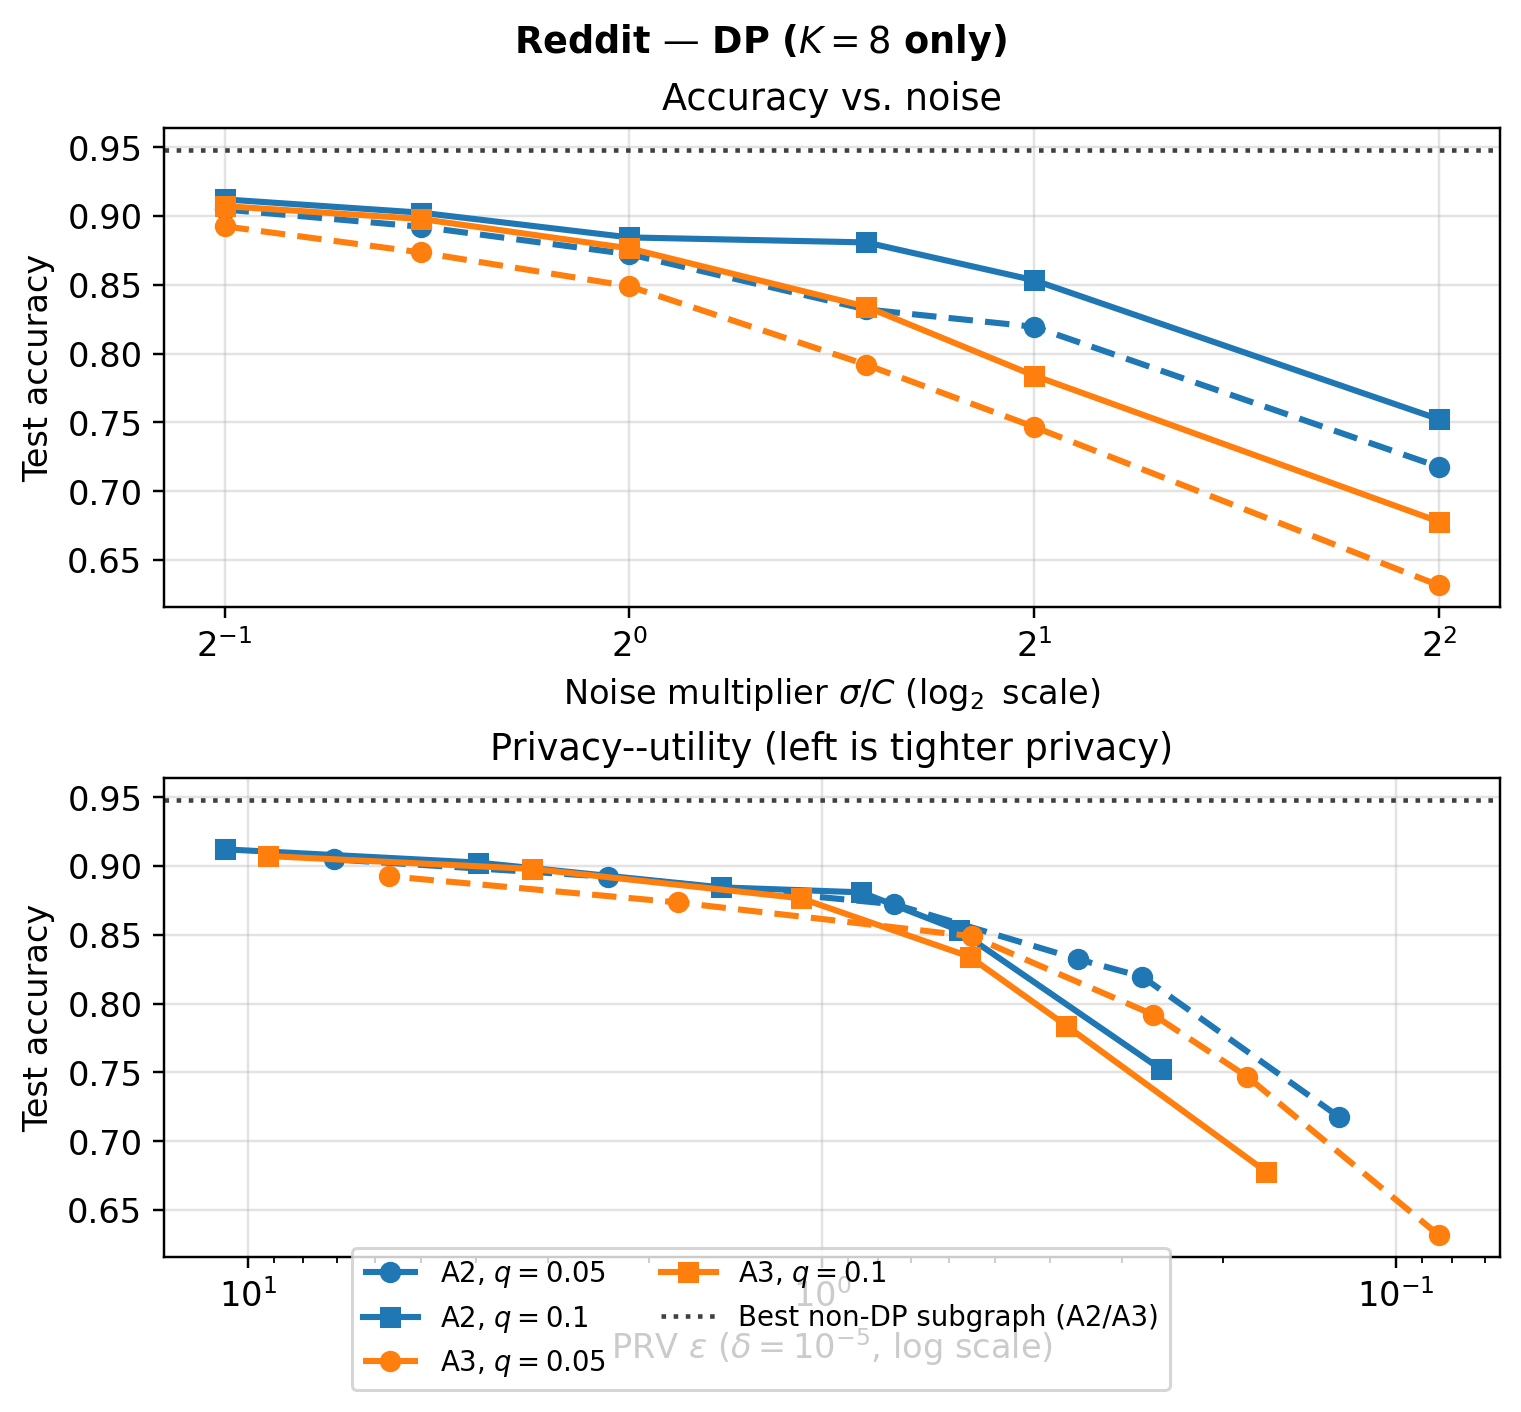
\includegraphics[width=\linewidth,height=0.30\textheight,keepaspectratio]{figures/experiments/dp_K8_reddit.png}
  \caption{\textbf{Reddit, $K{=}8$.} Same layout as Figure~\ref{fig:dp-k8-arxiv}.}
  \label{fig:dp-k8-reddit}
\end{figure}

\begin{figure}[htbp]
  \centering
  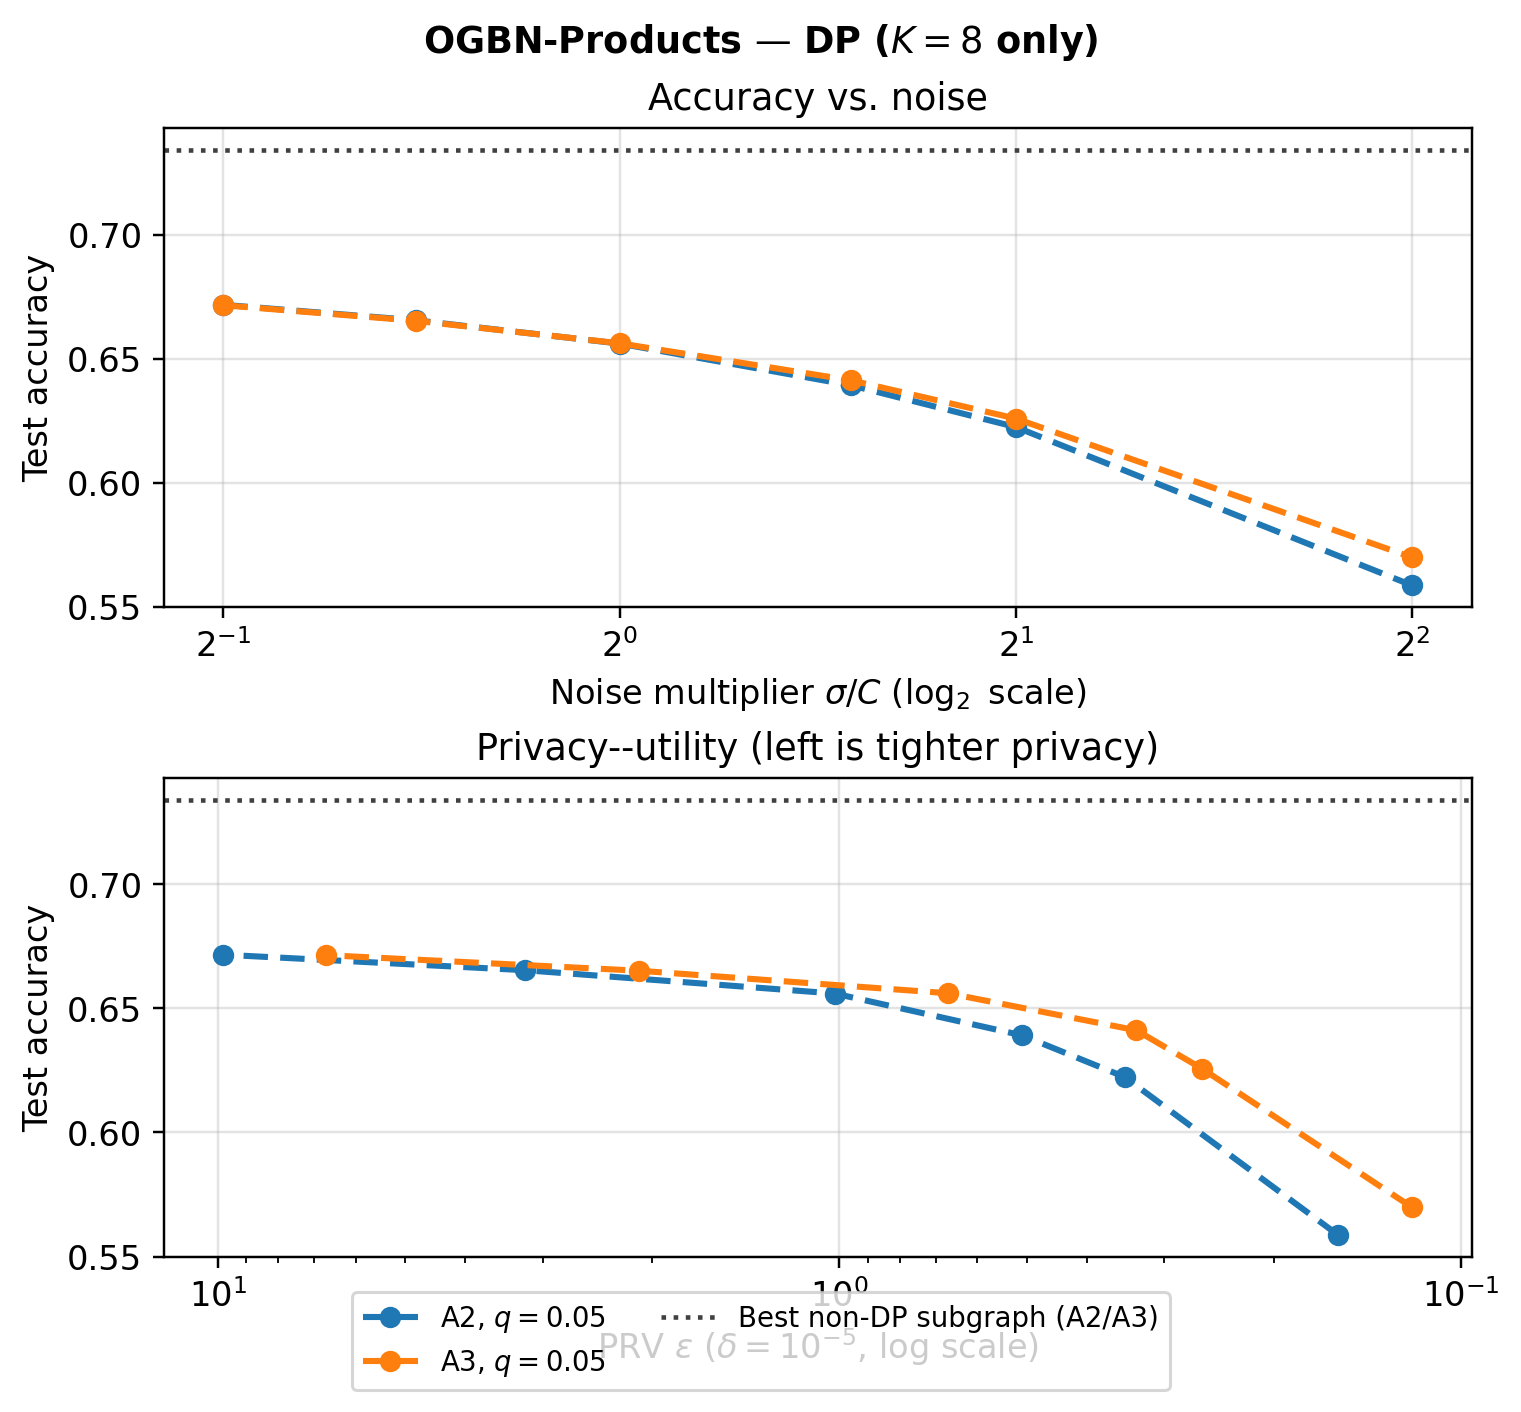
\includegraphics[width=\linewidth,height=0.30\textheight,keepaspectratio]{figures/experiments/dp_K8_ogbn_products.png}
  \caption{\textbf{OGBN-Products, $K{=}8$.} Same layout as Figure~\ref{fig:dp-k8-arxiv}.}
  \label{fig:dp-k8-products}
\end{figure}

\begin{table}[htbp]
  \centering
  \footnotesize
  \setlength{\tabcolsep}{4pt}
  \caption{DP at $\sigma/C{=}1$, $K{=}8$: test accuracy and PRV $\varepsilon$ for both~$q$ values.}
  \label{tab:dp-q}
  \begin{tabular}{lccccc}
\toprule
Dataset & $q$ & Algo.~2 acc. & Algo.~3 acc. & $\varepsilon$ (A2) & $\varepsilon$ (A3) \\
\midrule
\texttt{ogbn-arxiv} & 0.05 & 0.463 & 0.450 & 1.302 & 0.768 \\
\texttt{ogbn-arxiv} & 0.1 & 0.476 & 0.464 & 2.765 & 1.821 \\
\texttt{reddit} & 0.05 & 0.872 & 0.849 & 0.749 & 0.549 \\
\texttt{reddit} & 0.1 & 0.884 & 0.877 & 1.499 & 1.088 \\
\texttt{ogbn-products} & 0.05 & 0.656 & 0.656 & 1.018 & 0.669 \\
\bottomrule
\end{tabular}

\end{table}

% ---------------------------------------------------------------------------
\subsection{Effect of the number of bins~$K$ under DP}
\label{sec:exp-dp-K}

Finer partitions change both subgraph structure and the effective sampling rate per step ($q/K$ in single-phase accounting), so we report a compact table at a fixed privacy--noise operating point: $\sigma/C{=}1$ and $q{=}0.10$.
Table~\ref{tab:dp-K} contrasts $K\in\{4,8,16\}$ (Algos.~2 and~3); $\varepsilon$ differs across~$K$ because the same nominal noise is applied per bin while composition uses the reported step count.

\begin{table}[htbp]
  \centering
  \footnotesize
  \setlength{\tabcolsep}{3.5pt}
  \caption{DP at $\sigma/C{=}1$, $q{=}0.10$: test accuracy and $\varepsilon$ vs.\ $K$. Rows omitted if that setting is not yet present in the run logs (e.g.\ incomplete sweeps).}
  \label{tab:dp-K}
  \begin{tabular}{lccccc}
\toprule
Dataset & $K$ & Algo.~2 acc. & Algo.~3 acc. & $\varepsilon$ (A2) & $\varepsilon$ (A3) \\
\midrule
\texttt{ogbn-arxiv} & 4 & 0.458 & 0.432 & 6.832 & 3.781 \\
\texttt{ogbn-arxiv} & 8 & 0.476 & 0.464 & 2.765 & 1.821 \\
\texttt{ogbn-arxiv} & 16 & 0.492 & 0.484 & 1.209 & 0.860 \\
\texttt{reddit} & 4 & 0.893 & 0.879 & 3.832 & 2.651 \\
\texttt{reddit} & 8 & 0.884 & 0.877 & 1.499 & 1.088 \\
\texttt{reddit} & 16 & 0.901 & 0.871 & 0.757 & 0.539 \\
\bottomrule
\end{tabular}

\end{table}

% ---------------------------------------------------------------------------
\subsection{Reproducibility}

All numbers are generated from JSONL logs; rerun
\texttt{python scripts/plot\_headline\_results.py}
to refresh PNGs and table fragments.
Full dense sweeps over $(K,q,\sigma)$ remain in \texttt{dp\_runs\_summary.csv} for appendix material without cluttering the main text.
